\documentclass[11pt]{article}

\usepackage{../handout}
\usepackage{graphicx}

% Side margins:
% Actual margin is 1 in + this number
\oddsidemargin -0.25in
\evensidemargin -0.25in

% Text width:
\textwidth 6.9in

% Top margin:
% Actual margin is 1.5 in + this number
\topmargin -.3in

% Text height:
\textheight 8.7in

% Handout Numbers

\newcommand{\PAOneNum}{1}
\newcommand{\WAOneNum}{2}
\newcommand{\PATwoNum}{3}
\newcommand{\PAThreeNum}{4}
\newcommand{\WATwoNum}{5}
\newcommand{\WATwoSolNum}{6}
\newcommand{\WAOneSolNum}{7}
\newcommand{\WAThreeNum}{8}
\newcommand{\WAFourNum}{9}
\newcommand{\WAThreeSolNum}{10}
\newcommand{\PAFourNum}{11}
\newcommand{\WAFourSolNum}{12}
\newcommand{\WAFiveNum}{13}
\newcommand{\WAFiveSolNum}{14}
\newcommand{\WASixNum}{15}
\newcommand{\WASixSolNum}{16}
\newcommand{\PAFiveNum}{17}
\newcommand{\WASevenNum}{18}
\newcommand{\WASevenSolNum}{19}
\newcommand{\PAExtraNum}{20}
\newcommand{\WAEightNum}{21}
\newcommand{\WAEightSolNum}{22}
\newcommand{\PASixNum}{23}
\newcommand{\WANineNum}{24}
\newcommand{\WANineSolNum}{25}
\newcommand{\WATenNum}{26}
\newcommand{\WATenSolNum}{27}
\newcommand{\WAElevenNum}{28}
\newcommand{\WAElevenSolNum}{29}


\begin{document}
\handout{\WAOneSolNum}{2}{Solutions to Written Assignment 1}

\bigskip
\begin{enumerate}
	
	% #1
	\item DFAs for languages 
	\hspace*{1mm}
	\vspace{-6mm}
	\begin{center}
		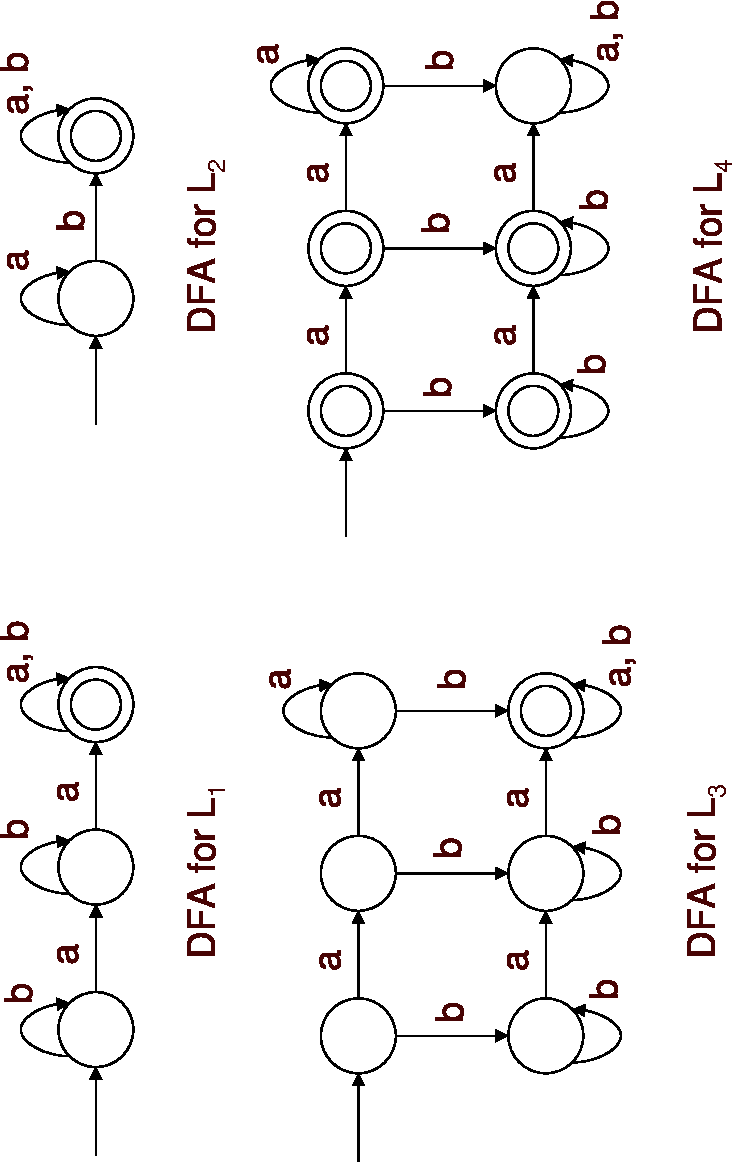
\includegraphics[height=3.7in,angle=-90]{wa1-q1-sol.pdf}
	\end{center}
	
	% #2
	\item DFAs and NFAs for languages
	\hspace*{1mm}
	\vspace{-4mm}
	\begin{center}
		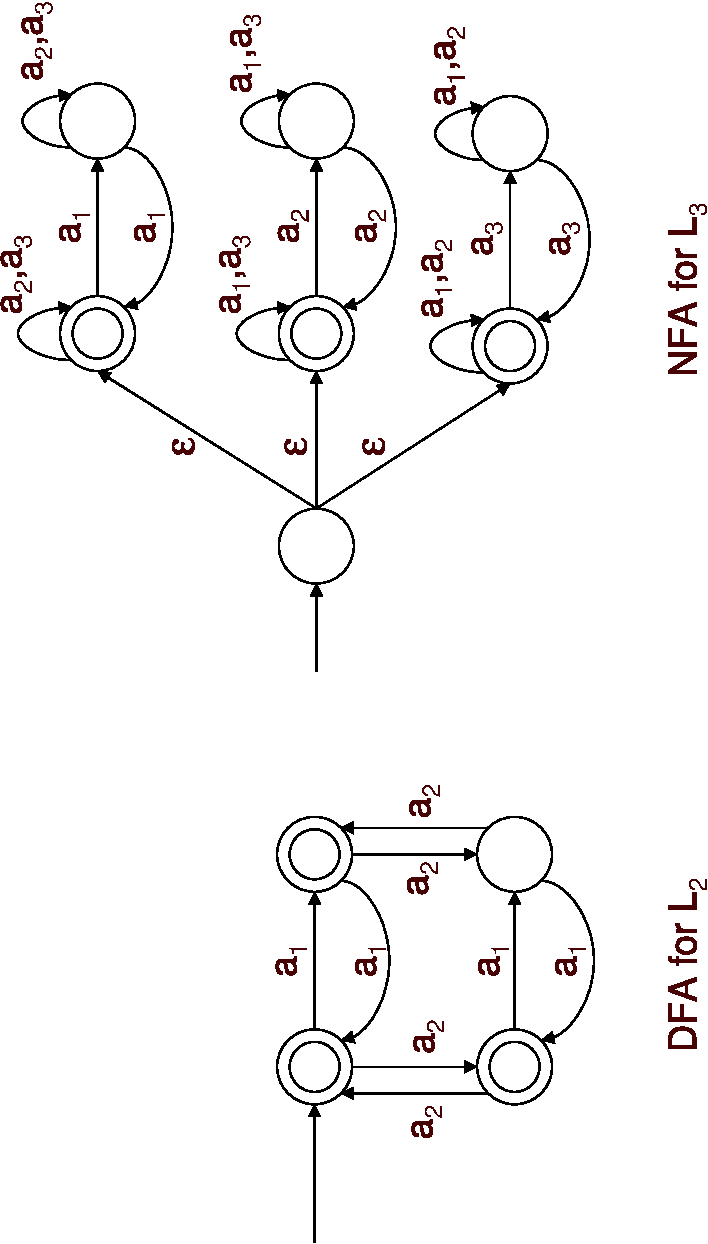
\includegraphics[height=4.5in,angle=-90]{wa1-q2-sol.pdf}
	\end{center}
	
	% #3
	\item Regular expressions
	\begin{enumerate}
		\item $(0 + 1)^*0(0 + 1)^*11$
		\item $\epsilon + 0 + 1 + (00 + 10 + 11)(0 + 1)^*$
		\item $0^*10^*(0^*10^*10^*)^*$
		\item $(00^* 1 0^* 1 0^*) + (0^* 1 00^* 1 0^*) + (0^* 1 0^* 1 00^*)$
	\end{enumerate}
	
	\newpage
	
	% #4
	\item Regular expression and description from DFA
	\begin{itemize}
		\item The language of all strings that begin and end with a 0 and have 
			an even, non-zero number of 1s (that is, $2k$ 1s, for some $k \ge 1$).
		\item $00^*10^*10^*(10^*10^*)^*0$
	\end{itemize}
	
	% #5
	\item Lexical analysis
	\begin{enumerate}
		\item An even length string of 0�s prints all a�s, while an odd length string of 
			0�s will have one c at the end (because of the maximal munch rule). Thus, 
			strings of 0�s generate the language $a^*c?$. Interspersed 1�s generate b�s, 
			so the full language is
			\begin{center}
				$(a^*c?b^+)^*a^*c?$
			\end{center}
			A common mistake might be to incorrectly account for the priority between the 
			rules for 0 and 00.
		\item Every input string can be divided into three sections (any of which might be empty)
			\begin{itemize}
				\item An initial string of 1s
				\item A section where a string of 0s is followed by a string of 1s, and this 
					pattern repeats (i.e., the language $((0+)(1+))^*$ )
				\item A final string of 0s
			\end{itemize}
			Thus, this specification can print any string in the language $c^*a^*b^*$.
	\end{enumerate}
	
\end{enumerate}
\end{document}
